\section{Actores}

A continuación se describen los actores que se involucran, de una manera u otra,
con el sistema.

\begin{description}

\item[Cliente] \hfill \\
Solicita una tarjeta y realiza compras con ella.

\item[Comercio] \hfill \\
Realiza ventas de bienes y/o servicios al cliente, quien paga por ellos
utilizando la tarjeta.

\item[Administrador] \hfill \\
Configura y adminstra el sistema informático desarrollado manteniendo datos de
referencia como ser los comercios y clientes registrados.

\item[Mensualmente] \hfill \\
Actor temporal mensual involucrado en los procesos de generación de resúmenes de
cuenta por clientes y resúmenes de saldo por comercio.

\item[Diariamente] \hfill \\
Actor termporal diario involucrado en los procesos de verificación y renovación
de tarjetas vencidas.

\end{description}

\section{Diagrama de casos de uso} \label{sec:diagrama_casos_uso}

En la figura~\ref{fig:modcasosuso:diagramacasos} se exponen los actores
involucrados en la operación del sistema y su interacción con el mismo a través
de los casos de uso identificados. En secciones subsiguientes se detallará cada
uno de estos últimos.

\begin{figure}[htb]
\begin{center}
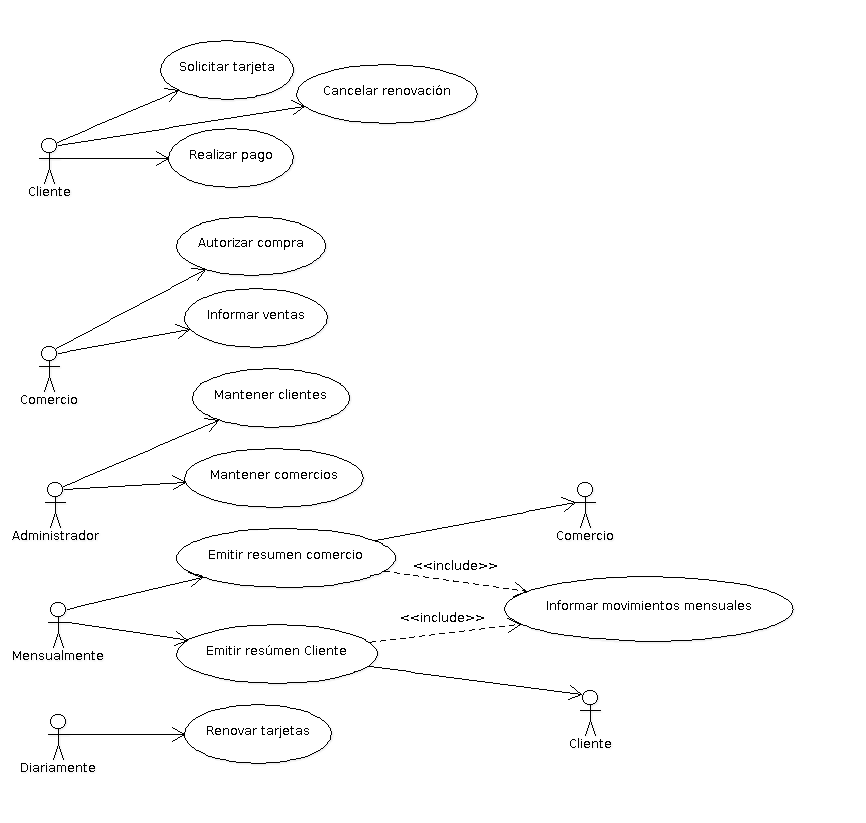
\includegraphics[width=0.9\textwidth]{images/mod_casosuso_diagrama.png}
\end{center}
\caption{Diagrama de casos de uso}
\label{fig:modcasosuso:diagramacasos}
\end{figure}

\FloatBarrier

\section{Detalle de casos de uso}

En esta sección se detallan cada uno de los casos de uso presentados en el
diagrama de casos de uso de la sección~\ref{sec:diagrama_casos_uso}.

\subsection{Solicitar tarjeta}
\begin{tabularx}{\textwidth}{| r | X |}
\hline
\multicolumn{2}{|X|}{
\textbf{Use Case}: Solicitar tarjeta} \\

\hline
\multicolumn{2}{|c|}{\cellcolor[gray]{0.6}} \\

\hline
\multicolumn{2}{|X|}{
\textbf{Descripción}: Registración de los datos de un cliente y emisión de una
tarjeta a su nombre.} \\

\hline
\multicolumn{2}{|X|}{
\textbf{Actores participantes}: Cliente} \\

\hline
\multicolumn{2}{|c|}{\cellcolor[gray]{0.6} } \\

\hline
\multicolumn{2}{|X|}{
\textbf{Flujos}} \\

\hline
\multicolumn{2}{|X|}{
\textbf{Flujo principal}} \\

\hline
1 & El cliente solicita una nueva tarjeta. \\
\hline
2 & El sistema solicita los datos del cliente. \\
\hline
3 & Se ingresan los datos del cliente (nombre, apellido, dni, límite de compra,
domicilio, teléfono). \\
\hline
4 & El sistema valida que el dni del cliente no haya sido registrado aún (E1.1
si ya ha sido registrado). \\
\hline
5 & El sistema pide confirmación de que el cliente ha presentado una fotocopia
de su dni (E2.1 si no se da confirmación). \\
\hline
6 & El sistema pide confirmación de que el cliente ha presentado la
documentación asociada a la garantía, y que esta es satisfactoria (E2.1 si no se
da confirmación). \\
\hline
7 & El sistema almacena los datos del cliente y genera un número de tarjeta. \\
\hline
8 & Fin del caso de uso. \\

\hline
\multicolumn{2}{|X|}{
\textbf{Flujos de excepción}} \\

\hline
E1.1 & El sistema emite un mensaje de error informando que el cliente ya posee
una tarjeta. \\
\hline
E1.2 & El caso de uso continua en 8 \\

\hline
E2.1 & El sistema emite un mensaje de error informando que el cliente no
presentó documentación obligatoria para continuar con la solicitud. \\
\hline
E1.2 & El caso de uso continua en 8 \\

\hline
\end{tabularx}



